\documentclass[../Bachelorarbeit.tex]{subfiles}
\begin{document}

\subsection{Verhaltensspezifikation}
Dieses Unterkapitel beschäftigt sich mit der Modellierung des Systemverhaltens. Anschließend an die Systemanalyse, ist die nun folgende Modellierung Teil der detaillierten Systemanalyse. Die Verhaltensspezifikation beinhaltet sämtliche Informationen zum Verhalten des gesamten Systems und dessen Systemprozesse. Als Basis dienen die in \autoref{AnwfallSpezPraez} dargestellten Anwendungsfallbeschreibungen. Ziel dieses Abschnittes ist es ein \bzw mehrere Zustandsdiagramme aus den Informationen der Anwendungsfallbeschreibungen zu entwickeln. Auf Grundlage der Tabellen aus dem vorhergegangenen Kapitel entsteht eine Verhaltensbeschreibung der zugrundeliegenden Systemprozesse. Zunächst erfolgt eine methodische erläuterung zur konstruktion eines solchen Zustandsdiagramms. \\
Die Konstruktion des Zustandsdiagrammes kann in folgende sieben Schritte untergliedert werden:
\begin{itemize}
    \item Zunächst müssen sämtliche Ereignisse \bzw wesentliche Schritte des Prozesses auf Unterbrechbarkeit geprüft werden. Unterbrechbare Elemente werden anschließend als \textbf{Aktivitäten} des Zustandsdiagramms modelliert. Ununterbrechbare Elemente sind als \textbf{Aktionen} des Zustandsdiagramms zu definieren.
    \item \textbf{Aktivitäten} werden in den Zuständen des Diagrammes abgebildet. Dazu wird eine solche Aktivität hinter dem Schlüsselwort \glqq do\grqq{} aufgeschrieben. Es ist hilfreich einen prägnanten Namen zu wählen. (Übergänge, die in den Zustand führen, sind aus dem Ereignis des jeweiligen Anwendungsfalldiagramms zu entnehmen.)
    \item \textbf{Aktionen} werden als Übergänge eingezeichnet und mit einem Ereignis beschriftet. (Am Ende eines Überganges wird die entsprechende Aktion eingezeichnet.)
    \item Verbleibende freie Enden \bzw Anfänge werden auf potentielle Start- oder Endzustände untersucht. Bei der Ermittlung eines solchen Zustands muss dieser entsprechend der Symbolik des Zustandsdiagramms mit dargestellt werden.
    \item Falls dennoch frei Übergangsenden verbleiben, müssen Zustände gefunden werden, auf welche diese verweisen. Zunächst sollten existierende Zustände geprüft werden. (Ein Ereignis kann auch an mehreren Zuständen hängen.) Wird kein Zustand gefunden, muss ein neuer Zustand erfunden werden.
    \item Es besteht die Möglichkeit Regionen oder auch zusammengesetzte Zustände zu definieren, um die Lesbarkeit zu erhöhen.
    \item Den letzten Schritt der Konstruktion stellt die Anreicherung der Übergänge mit \acp{nfa} dar. Dazu gehört unter anderem auch das Zeitverhalten aus den Anwendungsfallbeschreibungen. 
\end{itemize}

Die nun Folgenden Grafiken zeigen die Zustandsdiagramme zu den ermittelten Systemprozessen. Die Modellierung dieser folgt der zuvor beschriebenen Methodik. Auf Grund der starken Abweichungen des Systemverhaltens im Automatikmodus und im Handmodus, werden beide Betriebsmodi in getrennten Diagrammen dargestellt, auch wenn der zugrundeliegende Prozess gleich ist. 

\begin{figure}[h]
    \centering
    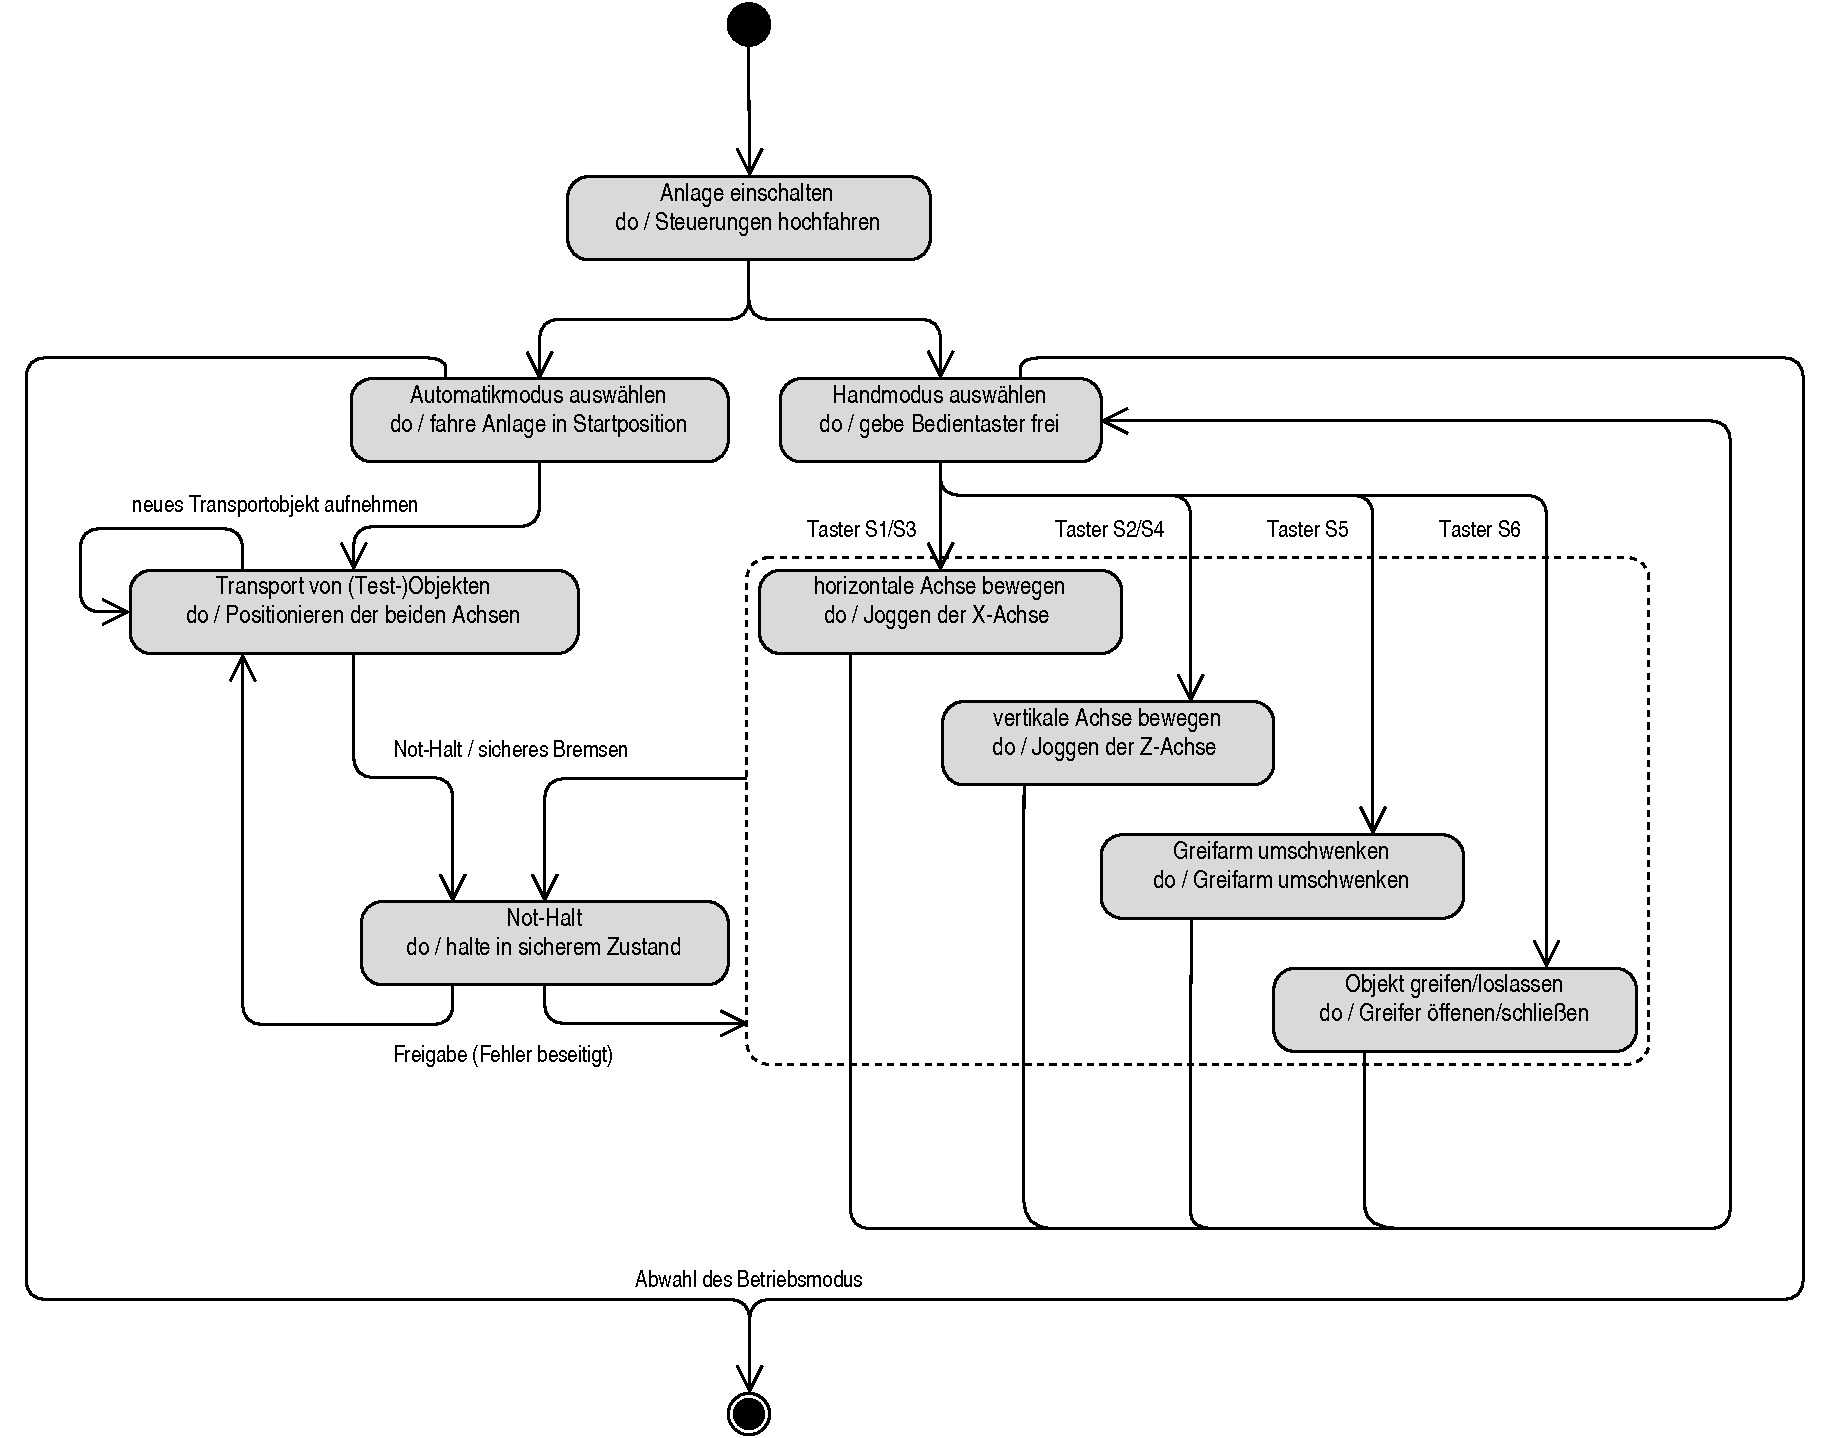
\includegraphics[width=\textwidth]{Images/zustandsdiagramm.pdf}
    \caption[Zustandsdiagramm]{Zustandsdiagramm - Systemprozess: Objekttransport}
    \label{fig:my-img4}
\end{figure}

\end{document}